\documentclass[12pt]{article}
\usepackage[utf8]{inputenc}
\usepackage[margin=1.1in]{geometry}
\usepackage{setspace}   %Allows double spacing with the \doublespacing command
\usepackage{amsmath}
\usepackage{graphicx}

\title{Linear Algebra in Population Modeling}
\author{Qingqing Yang, Adithya Shastry, Arunika Bhatia}
\date{May 10, 2019}

\begin{document}
\doublespacing
\maketitle
\newpage

\section{Overview}

Population modeling is a valuable branch of ecology, used by natural resource management groups such as the Bureau of Land Management (BLM). Population models seek to understand and explain changes in population size over time and predict population viability looking towards the future. These models can be used to tailor management interventions, such as prescribed burns or captive breeding, to stabilize population levels.

The field of population modeling was first created by biologists in the late eighteenth century. One of the first attempts to represent population growth was the geometric model, discovered by Thomas Malthus. After this, Francois Verhulst created the logistic growth model in 1838. Population modeling research experienced a resurgence in the 20th century when the human population began to place a strain on global food resources. Alfred J. Lotka and Vito Volterra soon created a paired differential equation model to quantify the relationship between predators, prey, and parasites. In 1939, Patrick Leslie used matrix algebra and life tables to calculate population growth accounting for life-stage. These models (geometric, logistic, Lotka-Volterra, and Leslie matrices) form the foundations of future population modeling \cite{national}

Life table graphs (life expectancy and mortality statistics) can be transcribed to population projection matrices.  Population projection matrices can then be used to determine population growth rates ($\lambda$) and manipulating the population projection matrix can be used to identify which elements of the matrix are most responsible for changes in the growth rate. In the matrix, each element represents a vital rate, with the first subdiagonal representing the survivorship probabilities (proportion of individuals surviving from one age group to the next) and the first row shows the fecundities (the average number of offspring had by each individual). Given data on population levels by age group and the population’s reproductive capacity, linear algebra can be applied to find the population growth rate and predict future population levels \cite{smith_geoff_ludwig_2011}.

\section{Age-Structured Model}

Age-structured population models are discrete models which use the fecundity and survival rates of each age class. Given the number of individuals at each age in one time step, we can calculate the number of individuals of each age in the next one. The average individual in each age group has a certain survivorship probability and fecundicity in that time. Ultimately, matrices and determinants are used to find the proportions of age groups are stable. 
\begin{figure}[h!]
  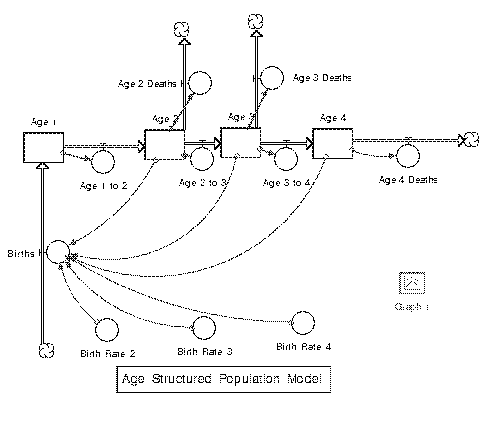
\includegraphics[width=\linewidth]{img.PNG}
  \caption{The interaction of birth and survival rates in an age structured population model}
  \label{model}
\end{figure}

\newpage
A Leslie matrix, $P$, is the matrix with the fecundity of each age class on the first row and their survival rates in the diagonal underneath (the first sub diagonal). Then, if $N_{t+1}$ and $N_t$ are the vectors representing the number of individuals in each age group at the times $t+1$ and $t$, then $N_{t+1}=PN_t$. In general, $N_{t+n}=(P^n)N_t$ \cite{vandermeer_goldberg_2013}. 


%[show P^n, which is (λ^n)I]. 

\begin{equation*}
    \textbf{P}=
    \begin{bmatrix}
    0&m_1&m_2&m_3&...&m_n\\
    p_{1,0}&0&0&0&...&0\\
    0&p_{2,1}&0&0&...&0\\
    0&0&p_{3,2}&0&...&0\\
    \vdots\\
    0&0&...&\dots&p_{n,n-1}&0\\
    \end{bmatrix}
\end{equation*}

Take, for example, a species with "babies", "middle-aged", and "old" individuals. Let us say the population begins with 10 old individuals. Assume that middle-aged individuals have a 50$\%$ survival rate and each middle-aged individual has 5 babies every time step. Assume, also, that old individuals have a 20$\%$ survival rate and each old individual has 10 babies every time step. Then, the Leslie matrix is as follows:

\begin{equation*}
    \textbf{P}=
    \begin{bmatrix}
    0&5&10\\
    0.5&0&0\\
    0&0.2&0\\
    \end{bmatrix}
    \end{equation*}
    
    So, starting from the initial distribution vector, the population at the seven consecutive time steps are as follows. They can be obtained by applying P recursively to the vectors seven times or by applying $P^7$ to the initial vector.
    
    
    

\begin{equation*}
    \begin{bmatrix}
    0\\
    0\\
    10
    \end{bmatrix}
    \xrightarrow{}
    \begin{bmatrix}
    100\\0\\0
    \end{bmatrix}
    \xrightarrow{}
    \begin{bmatrix}
    0\\50\\0
    \end{bmatrix}
    \xrightarrow{}
     \begin{bmatrix}
    250\\0\\10
    \end{bmatrix}
    \xrightarrow{}
     \begin{bmatrix}
    100\\125\\0
    \end{bmatrix}
    \xrightarrow{}
     \begin{bmatrix}
    625\\50\\25
    \end{bmatrix}
    \xrightarrow{}
     \begin{bmatrix}
    500\\312\\10
    \end{bmatrix}
    \xrightarrow{}
     \begin{bmatrix}
    1662\\250\\62
    \end{bmatrix}
    
    
\end{equation*}

Here, the equilibrium stage is achieved when the youngest age class is 76$\%$, the middle-aged class is 22$\%$, and the oldest age class is 2$\%$ of the population. So, if the population started at the following vector, these proportions would remain the same as time passes. Thus, the populations at equilibrium states are eigenvectors, and they are multiplied by the eigenvalue between time steps.

\begin{equation*}
     \begin{bmatrix}
    76\\22\\2
    \end{bmatrix}
\end{equation*}




When $t$ is adequately large and the population is at equilibrium (the relative proportions of the age classes are stable), $N_{t+1}= \lambda N_t$. Ecologists call the Leslie matrix the population projection matrix, but this term refers to forecasted populations rather than projection onto a vector space.

The stable age distribution shows the percentage of each age category that remains stable over increasing $t$. That is, for a stable distribution, each age category is increasing by the same factor: \textbf{$\lambda$}. If a model begins with a stable age distribution, the population of each age group will increase exponentially and smoothly, and, if a population does not, it will experience fluctuations before reaching a stable state. A population with constant mortality and constant natality must reach a stable age distribution at some $t$. Then, the finite rate of increase of a population equals the dominant (largest) eigenvalue of the Leslie matrix. The dominant (largest) eigenvalue of the Leslie matrix is the finite rate of increase of a population at equilibrium. However, this does not take into account the density dependence which limits most real populations. 

To derive the eigenvalues, we use the fact that, in general,

\begin{equation*}
    N_{t+1}=P(N_t)
\end{equation*}
And at equilibrium,
\begin{equation*}
    N_{t+1}=\lambda N_t
\end{equation*}
Therefore, at equilibrium,
\begin{equation*}
   PN_t=\lambda N_t
\end{equation*}
\begin{align*}
   PN_t-\lambda N_t&=0\\
   (P-\lambda I_n)N_t&=0
\end{align*}
Thus, in the $2 \times 2$ case,
\begin{equation*}
P-\lambda I_n=
    \begin{bmatrix}
    -\lambda&m\\
    g&-\lambda\\
    \end{bmatrix}
\end{equation*}
Where adults produce $m$ juveniles every time step, juveniles have survival rate $g$, and adults live for only one year.

\begin{align*}
    \det(P-\lambda I_n)=\lambda^2-gm&=0\\
\end{align*}

\begin{equation*}
        \lambda=\sqrt{gm}  
\end{equation*}
or
\begin{equation*}
   \lambda= \sqrt{-gm}
\end{equation*}

The largest root is the dominant eigenvalue, which represents the growth rate at equilibrium.

The addition of age structure in a population model is valuable because it allows us to consider different fecundity and survival rates of the age groups. However, this model can be further improved to account for density-dependence. Populations do not realistically grow exponentially without bound, and density-dependence or species interactions may help the model behave more accurately. Furthermore, this model is closed to migration, and it is typically used to count only females, as this makes assessing fecundity rates more straightforward. Finally, this model deals with equal time-steps, which renders the Leslie matrix difficult to deal with for certain life history strategies, such as long-lived trees whose survival rates vary greatly in their first years, but whose lifespans are so long that creating hundreds of equal time steps is cumbersome. In future investigations, it would be useful to learn about new models or alterations to this model which can account for these shortcomings.



\section{Two Species Model}
Many ecological models must incorporate two species. This can be achieved using linear algebra and more specifically eigenvalues, eigenvectors, and matrices. In this example we will be modeling coyotes and roadrunners. These two species can be modeled using the two equations below\cite{bretscher_2019}.


\begin{align}
    c(t+1)= 0.86c(t) + 0.08r(t)\\
    r(t+1)= -0.12c(t) + 1.14r(t)
\end{align}

If we express this equation as a matrix, we get the following:

\begin{equation*}
    \begin{bmatrix}
    c(t+1)\\
    r(t+1)
    \end{bmatrix}
    =\begin{bmatrix}
    0.86  &   0.08\\
    -0.12  &    1.14\\
    \end{bmatrix}
    \begin{bmatrix}
    c(t)\\
    r(t)  \\
    \end{bmatrix}
    =A\Vec{x}(t)
\end{equation*}

Now let us look at an example. Since the formula is recursive, we must substitute $\Vec{x}(t)$ into the formula for $\Vec{x}(t+1)$. For example, the population after 10 years of an initial distribution of $\Vec{x}_0(t)=\begin{bmatrix}100\\100\end{bmatrix}$, the $\Vec{x}(10)=A^{10}\Vec{x}_0\approx \begin{bmatrix}80\\170\end{bmatrix}$. 
    
We can look at another scenario: let's say $\Vec{x}_0(t)=\begin{bmatrix}100\\300\end{bmatrix}$. Then,

\begin{equation*}
    \Vec{x}(1)=A\Vec{x}_0
    =\begin{bmatrix}
    0.86  &   0.08\\
    -0.12  &    1.14\\
    \end{bmatrix}
    \begin{bmatrix}100\\300\end{bmatrix}
    =1.1\begin{bmatrix}100\\300\end{bmatrix}
    =1.1\vec{x}_0
\end{equation*}
Here we can see that since $\vec{x}_0$ is an eigenvector of the population matrix, we can find subsequent populations just by using the eigenvalue of $1.1$.  For example, 

\begin{equation*}
    \vec{x}(t)=
    \begin{bmatrix}
    c(t)\\
    r(t)  \\
    \end{bmatrix}
    =
    1.1^t\vec{x}_0
    =1.1^t\begin{bmatrix}100\\300\end{bmatrix}
    
\end{equation*}
 This is saying that the overall population of both species will increase by ten percent for every time step, $t$. 


Since we can have eigenvectors for the matrix A, we can represent other initial population vectors as linear combinations of the eigenbasis. This will allow us to simplify the calculations when modeling these populations. An example can be seen below.

Let $\vec{v_1}$ and $\vec{v_1}$ be eigenvectors of the matrix $A$,$c_1$ and $c_2$ are constants. 

\begin{align*}
     &A^{t}(\vec{x}(t))=A^t(c_1\vec{v_1}+c_2\vec{v_2})\\
     &=A^{t}c_1\vec{v_1}+A^{t}c_2\vec{v_2}\\
     &=\lambda_1^{t}\vec{v_1}c_1+\lambda_2^{t}c_2\vec{v_2}
\end{align*}
With this equation, it is easy to solve for the population distribution at any time $t$.
\bibliography{bib.bib} 
\bibliographystyle{unsrt}

\end{document}
